\documentclass[12pt, oneside]{book}
\usepackage[top=1in, bottom=1in, left=1.2in, right=1in, a4paper]{geometry}
\title{Graph Based Storage for Relational Databases}
\author{Adarsh Mohata, Ajith P S, Ashish Kedia, Sourabh Suman}

 \ifx\pdftexversion\undefined
 \usepackage[dvips]{graphicx}
 \else
 
 \usepackage[pdftex]{graphicx}
 \DeclareGraphicsRule{*}{mps}{*}{}
 \fi
\usepackage{url}
\usepackage{tabularx}
\usepackage{chapterbib}
\usepackage{hyperref}
\usepackage{lscape}
\usepackage{longtable}
\usepackage{float}
\usepackage{url}
\usepackage{amsmath}
\usepackage{multicol}
\usepackage{color}
\usepackage[utf8]{inputenc}
\usepackage{listings}
\usepackage{kbordermatrix}
\usepackage{fancyhdr}
\usepackage{caption}
\usepackage{chngcntr}
\usepackage{pdfpages}
\usepackage{amsmath}
\counterwithin{figure}{chapter}
\counterwithin{table}{chapter}
%\pagestyle{fancy}
\lhead{\leftmark}
\rhead{}
\cfoot{}
\rfoot{\thepage}
\raggedbottom
\renewcommand{\bibname}{References}
\newcommand{\project}{Graph Based Storage for Relational Databases}
\setcounter{secnumdepth}{4}
\setcounter{tocdepth}{4}

\definecolor{codegreen}{rgb}{0,0.6,0}
\definecolor{codegray}{rgb}{0.5,0.5,0.5}
\definecolor{codepurple}{rgb}{0.58,0,0.82}
\definecolor{backcolour}{rgb}{0.95,0.95,0.92}

\lstdefinestyle{mystyle}
{   language=bash,
    basicstyle=\ttfamily,
    morekeywords={peter@kbpet},
    alsoletter={:~\$},
    morekeywords=[2]{peter@kbpet:},
    keywordstyle=[2]{\color{red}},
    literate={\$}{{\textcolor{red}{\$}}}1 
	    {:}{{\textcolor{red}{:}}}1
	    {~}{{\textcolor{red}{\textasciitilde}}}1,
    backgroundcolor=\color{backcolour},	  
    commentstyle=\color{red},
    keywordstyle=\color{blue},
    numberstyle=\tiny\color{codegray},
    stringstyle=\color{codepurple},
    basicstyle=\footnotesize,
    breakatwhitespace=true,         
    breaklines=true,                 
    captionpos=b,                    
    keepspaces=true,                 
    numbers=left,                    
    numbersep=5pt,                  
    showspaces=false,                
    showstringspaces=false,
    showtabs=false,                  
    tabsize=4
}

\begin{document}
\begin{titlepage}
 \begin{center}
	\emph{A Project Report on} \\
\vspace{1cm}
\large
\textbf{\project} \\
\normalsize
\vspace{5mm}
\emph{Submitted by} \\
\vspace{5mm}
\textbf{Adarsh Mohata - 12IT03 - $VI$ Sem B.Tech} \\
\vspace{1mm}
\textbf{Ajith P S - 12IT04 - $VI$ Sem B.Tech} \\
\vspace{1mm}
\textbf{Ashish Kedia - 12IT14 - $VI$ Sem B.Tech} \\
\vspace{1mm}
\textbf{Sourabh Suman - 12IT82 - $VI$ Sem B.Tech} \\
\vspace{1cm}
\emph{Under the guidance of} \\
\vspace{1cm}
\textbf{Prof. Ananthanarayana V. S.} \\
\textbf{Dept of IT, NITK Surathkal} \\
\vspace{5mm}
\emph{in partial fulfillment for the award of the degree} \\
\vspace{5mm}
\emph{of} \\
\vspace{4mm}
\textbf{Bachelor of Technology} \\
\vspace{4mm}
\emph{in} \\
\vspace{4mm}
\textbf{Information Technology} \\
\vspace{5mm}
\emph{at} \\
\begin{figure}[H]
	\centering
	
\includegraphics[height=3.5cm]{pics/nitk_logo.jpg}
\end{figure}
\vspace{1cm}
\textbf{Department of Information Technology} \\
\vspace{5mm}
\textbf{National Institute of Technology Karnataka, Surathkal} \\
\vspace{5mm}
\text{February 2015}
\end{center}
\end{titlepage}

\thispagestyle{empty}
\pagenumbering{gobble}
\pagebreak
\begin{center}
\Large
\textbf{Department of Information Technology} \\
\normalsize
\textbf{National Institute of Technology Karnataka, Surathkal} \\
\vspace{1cm} \Large
\textbf{Minor Project} \\ \vspace{0.5cm}
\textbf{Mid Semester Evaluation (February 2015)}
\vspace{1cm}
\end{center}
Course Code : IT 399 \\
Course Title : Minor Project \\
Title of the Project : Graph based storage for Relational Databases \\
Details of Project Group : \\
\vspace{5mm}
\\
\begin{table}[h!]
  \begin{center}
   \begin{tabular}{ p{0.05\textwidth} | p{0.2\textwidth} | p{0.2\textwidth} | p{0.4\textwidth} }
      \hline
      \multicolumn{1}{|c|}{\textbf{S.No}} & \multicolumn{1}{c|}{\textbf{Name}} & \multicolumn{1}{c|}{\textbf{Register No.}} & \multicolumn{1}{c|}{\textbf{Signature with Date}} \\ \hline
      \multicolumn{1}{c}{} & \multicolumn{1}{c}{} & \multicolumn{1}{c}{} & \multicolumn{1}{c}{\hspace{4cm}}\\
      \multicolumn{1}{c}{1} & \multicolumn{1}{c}{Adarsh Mohata} & \multicolumn{1}{c}{12IT03} & \multicolumn{1}{c}{}\\
      \multicolumn{1}{c}{} & \multicolumn{1}{c}{} & \multicolumn{1}{c}{} & \multicolumn{1}{c}{}\\
      \multicolumn{1}{c}{2} & \multicolumn{1}{c}{Ajith P S} & \multicolumn{1}{c}{12IT04} & \multicolumn{1}{c}{}\\
      \multicolumn{1}{c}{} & \multicolumn{1}{c}{} & \multicolumn{1}{c}{} & \multicolumn{1}{c}{}\\
      \multicolumn{1}{c}{3} & \multicolumn{1}{c}{Ashish Kedia} & \multicolumn{1}{c}{12IT14} & \multicolumn{1}{c}{}\\
      \multicolumn{1}{c}{} & \multicolumn{1}{c}{} & \multicolumn{1}{c}{} & \multicolumn{1}{c}{}\\
      \multicolumn{1}{c}{4} & \multicolumn{1}{c}{Sourabh Suman} & \multicolumn{1}{c}{12IT82} & \multicolumn{1}{c}{}\\
      \multicolumn{1}{c}{} & \multicolumn{1}{c}{} & \multicolumn{1}{c}{} & \multicolumn{1}{c}{}\\
   \end{tabular}

  \end{center}

\end{table}
\\
\\
\begin{tabular}{l@{\hskip 4cm} r}
	\line(1,0){150} \\
	 Prof. Ananthanarayana V. S. \\
	 Dept. of IT, NITK \\
	 Project Mentor \\ 
\end{tabular}

\vspace{4cm}
\begin{flushleft}
Place: NITK Surathkal, Mangalore \\
Date: \today
\end{flushleft}
\pagebreak
\thispagestyle{empty}
\begin{center}
	\textbf{ \huge Abstract}
\end{center}
\vspace{1cm}
Relational Database Management System has been there for quite a few decades. Relational databases are still the most popular means of storing huge amount of data on disk. They are efficient in most cases however in certain types of queries like Join they fail to compute the results efficiently. In recent times, quite a bit of research has been done on Graph Databases - which seems like a promising solution to the bottleneck. Many implementations of such databases have come up - Google's Cayley, Neo4j, etc. However even these graph databases suffer from several overheads.
\par
This project aims at exploring the various ways of using a graph-like storage model for traditional Relational Databases. \\
\par
\textbf{Keywords : }Database, Graph, Relational

\thispagestyle{empty}
\listoffigures
\tableofcontents

\setcounter{page}{1}
\pagenumbering{arabic}

\chapter{Introduction}
As the name suggests, graph database model uses graph structures for semantic queries with nodes, edges, and properties to represent and store data. A graph database storage system provides index-free adjacency. This means that every element contains a direct pointer to its adjacent elements and no index lookups are necessary.
\section{Motivation}
Graph Databases look like a promising model to solve all the problems that exist with the current relational databases. They provide an optimal way to compute the equivalent of the join query in a relational database. Recently there has been increased interest in graphs to represent social networks, web site link structures, and others. Within the field of biology itself, there are many uses for graphs, including metabolic networks, protein-protein interaction networks, chemical structure graphs, gene clusters, and genetic maps. Graphs truly are one of the most useful structures for modeling objects and interactions. However, Graph databases have their own overheads and drawbacks. Sometimes it is very difficult or even impossible to construct the equivalent relational database from a graph database. Moreover, graph databases don't use SQL and as such it is very difficult for the programmers to realize the query they want to perform. \\
\par
Owing to these reasons, the use of graph databases is currently limited. We were motivated to resolve this problem by taking a middle path between graph and relational databases. We wanted to explore the various ways to optimize the query execution time as well as the storage of the currently popular relational databases. We also wanted to eliminate some sort of data redundancy in a typical relational database system.
\begin{figure}[h]
 \begin{center}
  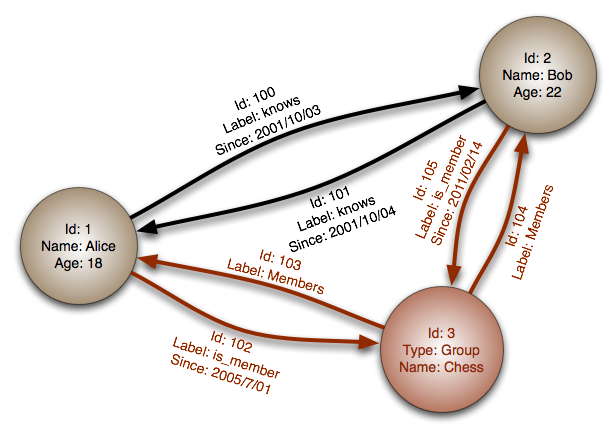
\includegraphics[width=\textwidth]{pics/graph.png}
  \caption{A Graph Database}
 \end{center}
\end{figure}

\pagebreak

\chapter{Literature Review}
Relational Databases are a common choice for primary data storage structure in both academic and commercial pursuits since the 1970s. The Relational Model organizes data into one or more tables of rows and columns, with a unique key for each tuple. Generally, each entity type described in a database has its own table, the tuples representing instances of that entity and the columns representing the attribute values describing each instance. They provide relational operators to manipulate the data in tabular form. Most of the relational databases use SQL as their query language. Relational database systems are generally efficient unless the data contains many relationships requiring joins of large tables. These costly join operations are usually addressed by denormalising data to reduce the number of joins necessary.  
\section{Graph Model}
In recent years, software developers have been investigating storage alternatives to relational databases. BigTable, Cassandra, CouchDB, Project Voldemort, and Dynamo are all NoSQL projects, as they are all high-volume data stores that actively reject the relational model. In the graph model, nodes represent entities. Properties are pertinent information that relate to nodes. Edges are the lines that connect nodes to nodes or nodes to properties and they represent the relationship between the two. Compared with relational databases, graph databases are often faster for associative data sets and map more directly to the structure of object-oriented applications. They can scale more naturally to large data sets as they do not typically require expensive join operations. As they depend less on a rigid schema, they are more suitable to manage ad hoc and changing data with evolving schema. Graph databases are a powerful tool for graph-like queries, for example computing the shortest path between two nodes in the graph.\\
\par
However, relational databases are typically faster at performing the same operation on large numbers of data elements. A relational database is much faster when operating on huge numbers of records. In a graph database, each record has to be examined individually during a query in order to determine the structure of the data, while this is known ahead of time in a relational database. Relational databases use less storage space, because they don't have to store all of those relationships.

\section{Problem Statement}
To develop a data storage system based on graph structure in order to optimize the query execution time especially join queries and eliminate some sort of data redundancy in a relational model while retaining other advantages of relational database system in terms of performance of other queries.  

\section{Research Objectives}
\begin{itemize}
 \item To explore the pros and cons of the graph model.
 \item To compare the relational model with the graph model.
 \item To develop a model which can represent relational database.
 \item To define relational algebraic operations on the model such that it has most of the advantages of both the models.
 \item To understand the differences of the proposed model with the graph model.
 \item To realize the limitations of the proposed model.
\end{itemize}

\chapter{Methodology}
Relational databases performs inefficiently when you make a join type query. Graph database is able to perform join type queries quite fast because it stores the data using a graph structure. But because of the model used, it is sometimes unable to represent all kinds of relational databases. Realizing that the problem lies with the model of the graph used, we came up with our own model to represent relational databases, using graphs.\\

\par The model for a single relation can be represented as follows :
\begin{itemize}
 \item Each attribute of a relation will have its own domain.
 \item Each domain has a list of nodes called attribute nodes
 \item Each attribute node represents a particular value which exists in at-least one tuple's corresponding attribute. Note that a particular value belonging to a domain will only be represented once in the attribute list.
 \item We also have a main domain which too has a list of nodes, called main nodes.
 \item Each main node has as many links as the number of attributes in the relation.
 \item Each link will connect a particular domain's attribute node and the main node. No two links from the main node will connect to the same domain. The links connect to those attribute nodes which represent the value of the tuple's attribute.
\end{itemize}
When multiple relations are involved with some of them having foreign key relation, then our model will be expanded slightly to accommodate that as follows.\\
\par Suppose relation 1 has a foreign key relationship with relation 2. Then relation 1 is said to be the child and relation 2 is said to be the parent relation. Each tuple in the child relation will reference a single tuple in the parent relation. Multiple tuples can refer to the same tuple in the parent relation. In our model we add a single link between each main node of the child relation(Note that each main node represents a single tuple) and the main node in the parent relation to which it refers to.

\chapter{Work Done}
As of now we have been able to partially implement the proposed graph like storage.
\section{Implementation}
We have implemented the functionalities to create a table, insert records to it and index the records for faster retrieval. As of now we have only considered String data type.
\subsection{Indexing}
Trie is the optimal indexing methodology that returns that maps a string to it's corresponding node in the graph. The algorithmic complexity of inserting and querying a string in trie is $\mathcal{O} \left( d\right)$ where, $d$ is the length of the string mapped. The data structure can be further optimized in terms of storage requirements by using a compressed trie. However, for time bound remains optimal.
\par
The \emph{trie} class in the source code provides all the properties and functions required to index string data.
\subsection{Code Structure}
The Code is divided into multiple files for ease of development. Each file provides one or more classes that are a logical entity. The details have been discussed in the following section :
\begin{enumerate}
 \item \textbf{Database} - The database class is the root class that contains all the data. It only contains a list of all the tables. Currently the system supports only one database. It provides functionalities to add a new table, compute the size of all tables and delete all the tables on demand.
 \item \textbf{Table} - The table class represents a table. It provides (or will provide in future) all the table related functionalities like measuring size, inserting, selecting, projecting, etc. It also provides a function to delete the table on demand.
 \item \textbf{Main Node} - This class represents a typical tuple in a table. Although no data is stored in Main Node but it points to corresponding attribute node. A Linked List of main nodes make up a Table
 \item \textbf{Domain} - It represents the domain of a data. It is a linked list of all the valid values that an attribute can take. It provides functionality like searching, adding and deleting attribute nodes. It also provides function to measure storage requirements.
 \item \textbf{Attribute Node} - It is the smallest logical entity that stores the actual data. Only one copy of a particular value is stored in a domain to avoid redundancy. It also stores a list of pointers to all the records that are pointing to it.
 \item \textbf{Others} - Other classes such as primary and foreign key are also there however they are currently not been used.
\end{enumerate}
\section{Results}
The Results of out study can be divided into two sections - Storage and Time. We have performed both theoretical and well as practical memory bound calculations. \\
\subsection{Theoretical Calculations}
Each of the record in the graph storage has following extra data :
\begin{itemize}
 \item Pointer from Main Node to each Attribute Node
 \item Pointer from each Attribute Node to Main Node
 \item Pointer from one Attribute data to the next Attribute data (Next Pointer of linked list)
 \item Pointer from one main node to next main node in the table (Next Pointer of the Linked List)
\end{itemize}
Thus the size occupied by a table in the graph model can be equated using the following equation :
\begin{equation}
  Size\_Graph = (n * x * rs) + (n * ptr * (3 * attr + 1))
  \label{grsize}
\end{equation}
where, \\
$Size\_Graph$ = Size occupied by Graph Storage Engine, \\
$x$ = Fraction of tuples that are unique, \\
$rs$ = Theoretical size of each tuple in a table, \\
$n$ = Number of records in a table, \\
$attr$ = Number of Attributes in the table, \\
$ptr$ = Size of a pointer variable \\

The above equation illustrates the growth of database on the proposed graph storage engine. For a traditional Relational Database the space occupied by the data in the memory can be arrived at using the following equations :
\begin{equation}
 Size\_RDBMS = n * rs
 \label{rdbmssize}
\end{equation}
where, \\
$Size\_RDBMS$ = Size occupied by the Relational Database Engine, \\
$n$ = Number of tuples in a table, \\
$rs$ = Theoretical size of each tuple in a table \\

\par
Using equation ~\ref{grsize} and ~\ref{rdbmssize} we can conclude that given a particular table (Fixed number of attributes) on a particular system (Fixed Pointer Size) the Space complexity of both the engines is same i.e., $\mathcal{O}\left( n\right)$ where, $n$ is the number of tuples in the table. However, for absolute measurement we can equate the two equation to obtain a break-even point after which the graph storage engine is more efficient than the traditional relation model. 
\begin{center}
  \begin{math}
    (n * x * rs) + (n * ptr * (3 * attr + 1)) < n * rs
  \end{math}\\
  \begin{math}
    ptr * (3 * attr + 1) < rs * (1 - x)
  \end{math}
\end{center}
Assuming a typical record size to be 400 bytes, number of attributes to be 5, pointer size to be 8 bytes (x64 systems) we get,
\begin{center}
 \begin{math}
  8 * (3 * 5 + 1) < 400 * (1 - x)
 \end{math} \\
 \begin{math}
  128 < 400 * (1-x)
 \end{math} \\
 \begin{math}
  x < 0.68
 \end{math}
\end{center}
which means that if at-least 32\% of values in a table are repeated then the graph storage engine occupies less space than the relational databases. In a real-life database there numerous duplicate entries and thus the proposed storage model may perform better.

\subsection{Practical Observation}
We created an equivalent table in both a traditional RDBMS and our graph storage. We measured the size occupied by both the models. We have plotted several graphs. All this testing was done using a single table with 4 attributes and size of each attribute to be 80 bytes. Numbers of records are increasing along X axis, while space occupied by the model is increasing along Y axis.
\begin{enumerate}
 \item \textbf{100 Records} - Number of records was varied between 1 to 100. Observations were made after every record.
 \begin{figure}[H]
  \begin{center}
   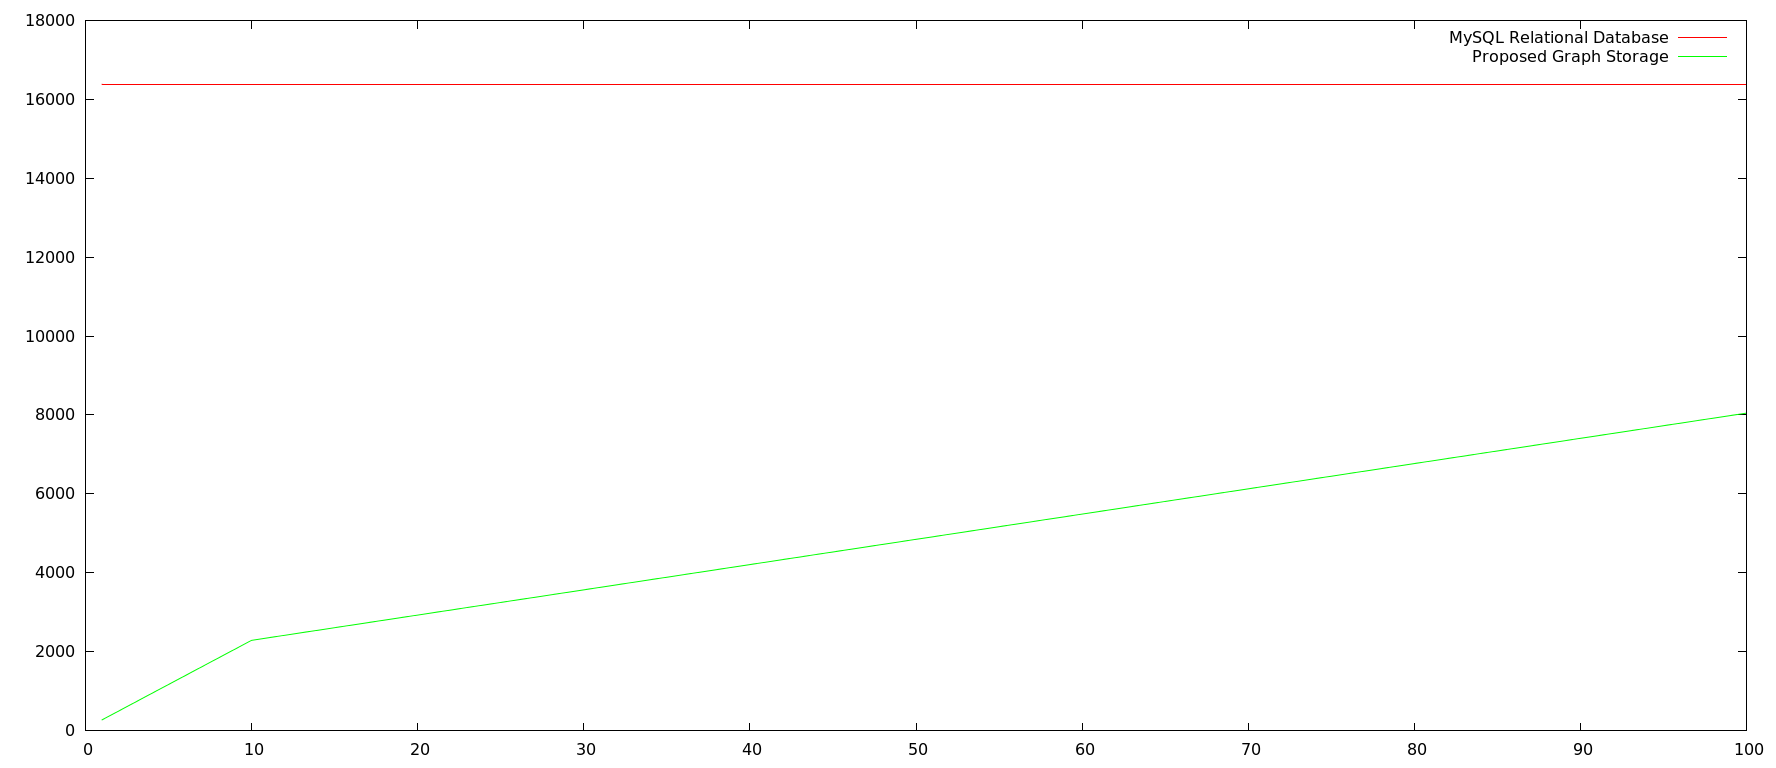
\includegraphics[width=\textwidth]{pics/100.png}
   \caption{Comparison of Size of 100 records}
   \label{100pic}
  \end{center}
 \end{figure}
\item \textbf{1000 Records} - Number of records was varied between 1 to 1000. Observations were made after every 10 record.
 \begin{figure}[H]
  \begin{center}
   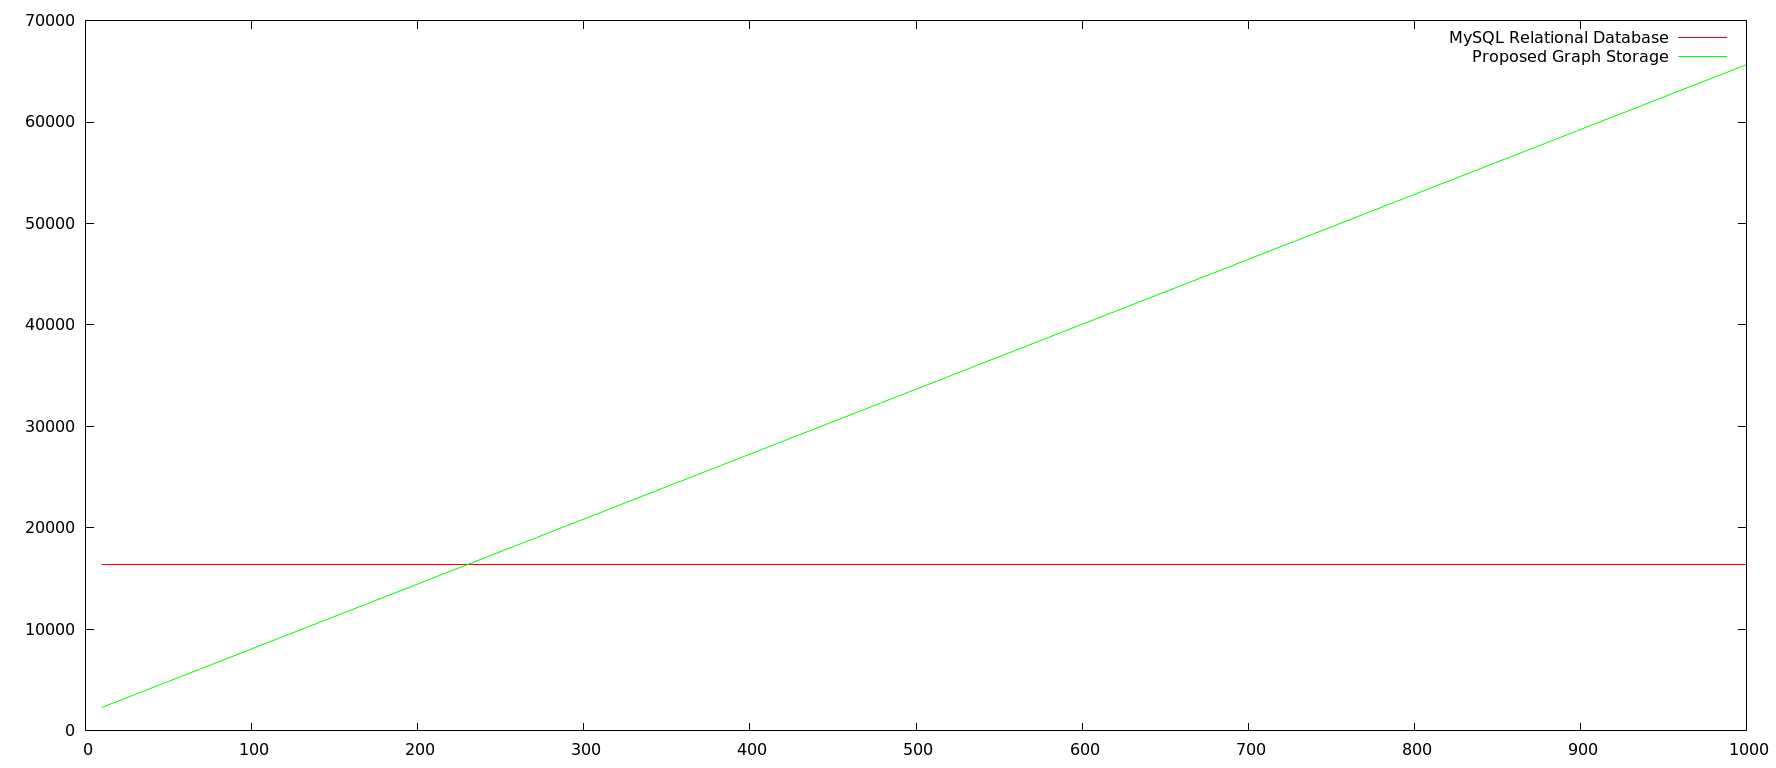
\includegraphics[width=\textwidth]{pics/1000.png}
   \caption{Comparison of Size of 1000 records}
   \label{100pic}
  \end{center}
 \end{figure}
\item \textbf{10000 Records} - Number of records was varied from 1 to 10000. Observations were made after every 100 record.
 \begin{figure}[H]
  \begin{center}
   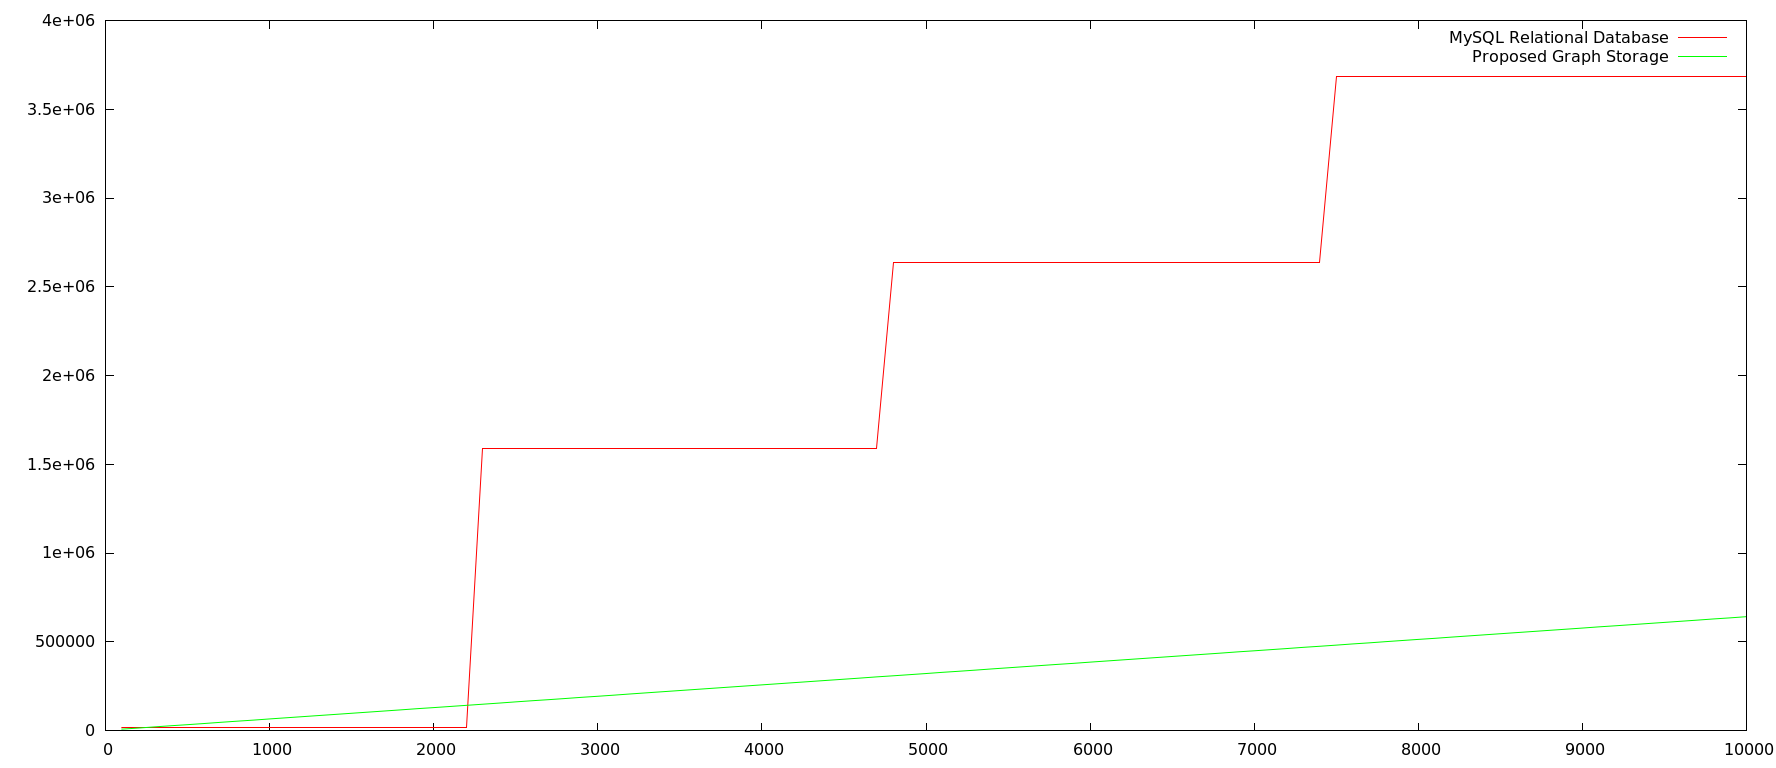
\includegraphics[width=\textwidth]{pics/10000.png}
   \caption{Comparison of Size of 10000 records}
   \label{100pic}
  \end{center}
 \end{figure}
 \item \textbf{100000 Records} - Number of records was varied from 1 to 100000. Observations were made after every 1000 record.
 \begin{figure}[H]
  \begin{center}
   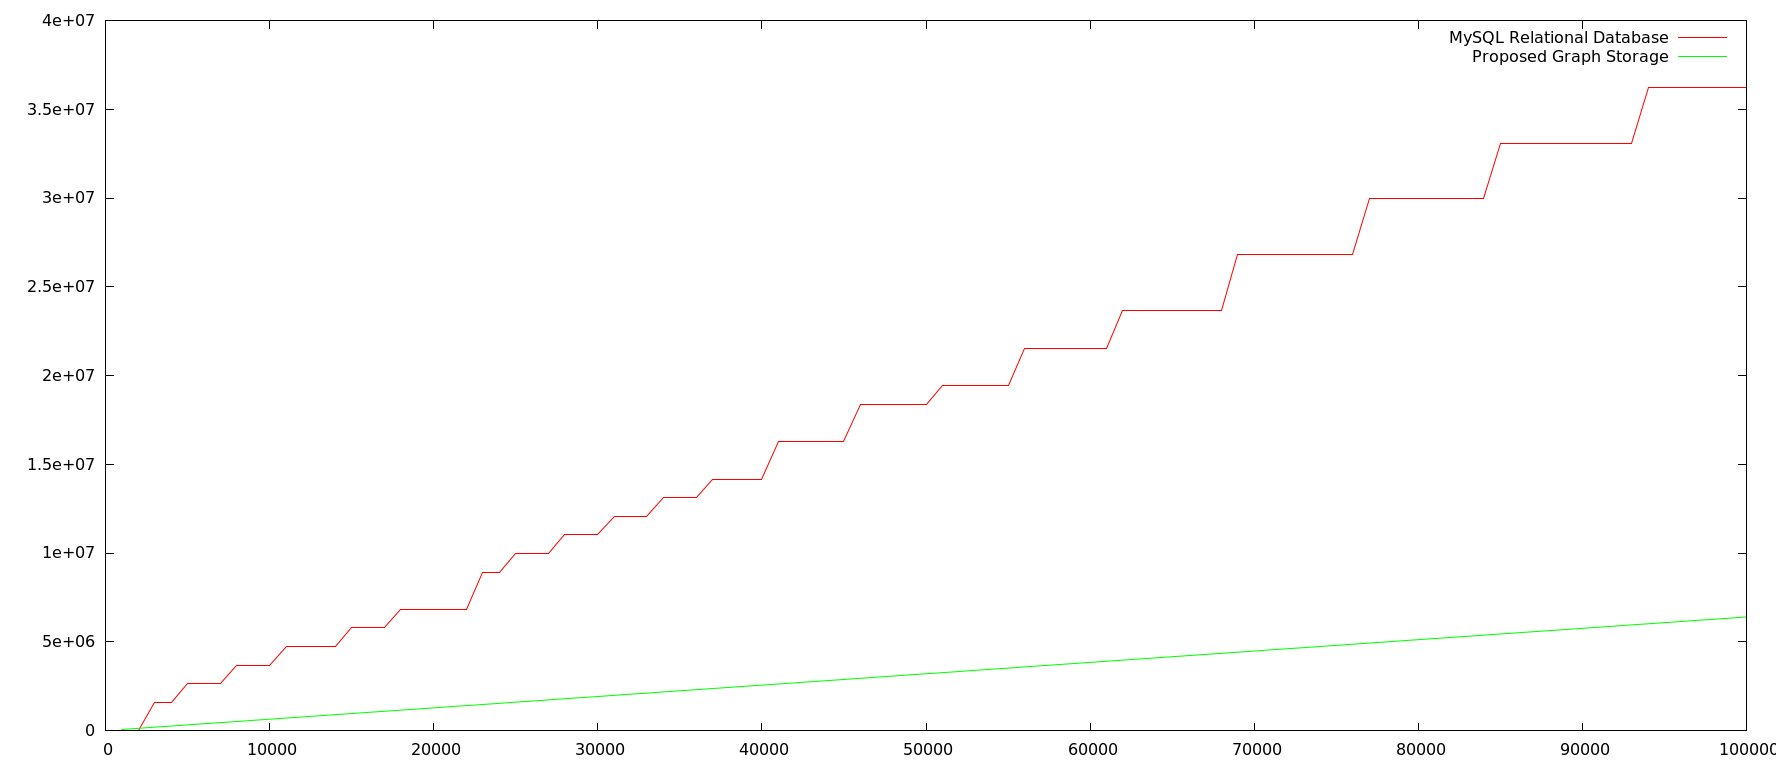
\includegraphics[width=\textwidth]{pics/100000.png}
   \caption{Comparison of Size of 100000 records}
   \label{100pic}
  \end{center}
 \end{figure}
\end{enumerate}
\par
It is clearly evident from these plots that traditional RDBMS increases their storage space in steps. In the long run the graph model performs better.
\par
However, Several factors were not accounted while making these observation - which makes these observations a little less reliable. We intend to perform a more vigorous analysis of the storage requirement in future.

\pagebreak

%\bibliographystyle{ieeetr}
%\bibliography{biblio}
%\addcontentsline{toc}{chapter}{Bibliography}
%\addcontentsline{toc}{chapter}{Appendix Paper 1}
%\includepdf[pages={1-9}]{paper1.pdf}
%\addcontentsline{toc}{chapter}{Appendix Paper 2}
%\includepdf[pages={1-6}]{paper2.pdf}
\end{document}